\subsection{\SubsecOnlineNesting} \label{subsec:nest_online}
%----------------------------------------------------------

オンライン・ネスティング実行時の制約として、
親領域と子領域の積分時間は一致している必要があり、
かつ、親領域の時間ステップは子領域の時間ステップの倍数でなければならない。
一方、親領域と子領域の間で鉛直層数、鉛直レベル、地図投影法、物理スキームは一致している必要はない。

オンライン・ネスティング実験では全ての領域の計算を同時に実行する。
現在は、親領域から子領域に対してデータの受け渡しを行う、一方向ネスティングのみをサポートしている。
オンライン・ネスティング実験でサポートするネスティングの段数は、最大で10段までである。

\scalerm のオンライン・ネスティング実験は、
複数の領域を逐次的に時間積分計算を進めるのではなく、並列的に時間積分計算を行う。
図\ref{fig_mpisplit}に示すイメージ図のように、
与えられたMPIプロセスを分割してそれぞれの領域に分配し、
各々の領域が独立したモデルのように計算を進める。
後ほど説明するが、複数の領域を立ち上げるために実行時には\verb|launch.conf|という
起動用の設定ファイルが別途必要になる。

\begin{figure}[ht]
\begin{center}
  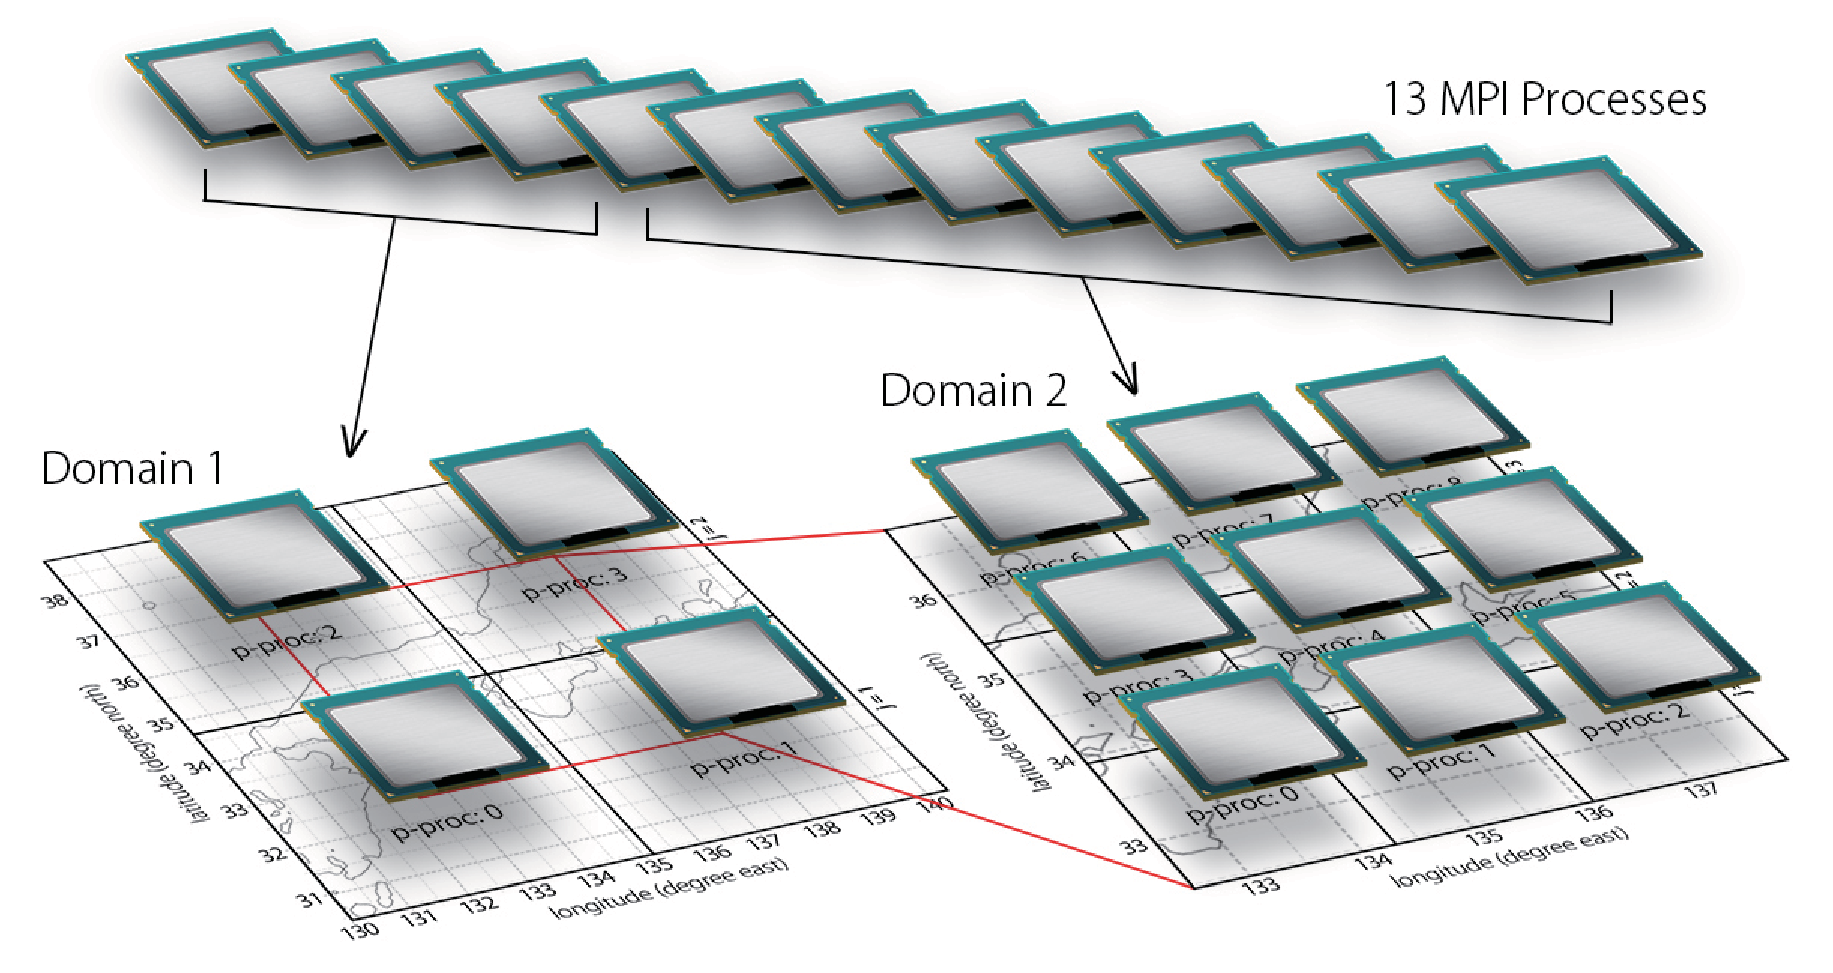
\includegraphics[width=0.8\hsize]{./figure/mpisplit_nesting.eps}\\
  \caption{オンライン・ネスティング実験のMPIプロセス配分イメージ. 全部で13のプロセスを立ち上げ、これを適切に分配することで、
           Domain 1は$2 \times 2$の4-MPI並列、Domain 2は$3 \times 3$の9-MPI並列計算を行う。Domain 1からDomain 2へMPI通信
           によってデータを受け渡ししながら時間積分計算を進める。}
  \label{fig_mpisplit}
\end{center}
\end{figure}


オンライン・ネスティングに必要な設定は複数ある他、設定の不具合があると計算が正常に行われない。
設定の詳細は以下の説明を参照することとし、実際の設定ファイル(\verb|**.conf|)は
第\ref{sec:basic_makeconf}節で説明する実験セット作成サポートツールで作成すること。


ここでは、最も単純な2段ネスティングの例を説明する。
オンライン・ネスティング実験を行う場合は、\verb|scale-rm|のモデル本体実行前に全ての領域について、
地形/土地利用データの作成、及び初期値/境界値データの作成を事前に行っておく必要がある。
従って、親領域と子領域それぞれについて、
\verb|pp.***.conf|、\verb|init.***.conf|、そして\verb|run.***.conf|ファイルを事前に作成し、
親領域、子領域ともに地形/土地利用データの作成、
及び初期値/境界値データの作成を終えていることを想定して説明を進める。
ここで説明するオンライン・ネスティング実験の設定を記述した設定ファイルが
\verb|${Tutorial_dir}/real/sample/online_nesting|に置いてあるので、
説明を読み進める上で参考にしてもらいたい。


\subsubsection{設定ファイルの編集}
まず、親領域、子領域それぞれに\verb|run.***.conf|ファイルを編集する。

\noindent {\gt \verb|run.parent.conf|の編集内容}\\
{\small {\gt
\ovalbox{
\begin{tabularx}{140mm}{l}
\verb|&PARAM_NEST| \\
\verb| USE_NESTING              = .true.,| \\
\verb| OFFLINE                  = .false.,| \\
\verb| ONLINE_DOMAIN_NUM        = 1,| \\
\verb| ONLINE_IAM_PARENT        = .true.,| \\
\verb| ONLINE_IAM_DAUGHTER      = .false.,| \\
\verb| ONLINE_BOUNDARY_USE_QHYD = .true.,| \\
\verb| ONLINE_AGGRESSIVE_COMM   = .true.,| \\
\verb|/| \\
\end{tabularx}
}}}\\

\vspace{0.5cm}

\noindent {\gt \verb|run.child.conf|の編集内容}\\
{\small {\gt
\ovalbox{
\begin{tabularx}{140mm}{l}
\verb|&PARAM_NEST| \\
\verb| USE_NESTING              = .true.,| \\
\verb| OFFLINE                  = .false.,| \\
\verb| ONLINE_DOMAIN_NUM        = 2,| \\
\verb| ONLINE_IAM_PARENT        = .false.,| \\
\verb| ONLINE_IAM_DAUGHTER      = .true.,| \\
\verb| ONLINE_BOUNDARY_USE_QHYD = .true.,| \\
\verb| ONLINE_AGGRESSIVE_COMM   = .true.,| \\
\verb|/| \\
\end{tabularx}
}}}\\

\noindent 上記の\namelist{PARAM_NEST}の項目は、ネスティング実験のために新たに加える項目である。
もともとの設定ファイルには項目自体がないので、自分で設定ファイルに追記する。最初の2つの項目
\nmitem{USE_NESTING = .true., OFFLINE = .false.}によって、
オンライン・ネスティング実験であることが決定される。
\nmitem{ ONLINE_}で始まる設定変数はオンライン・ネスティング実験
専用の設定変数である。\nmitem{ONLINE_DOMAIN_NUM}は、
領域のID番号であり、外側領域から内側領域へ順番に
番号を振っていく。ここでは、親領域は1番、子領域は2番と設定する。

\nmitem{ONLINE_IAM_PARENT}と\nmitem{ONLINE_IAM_DAUGHTER}は各領域の役割を設定するパラメータである。
これらの変数は、``In online nesting system, I am parent (or, I am child).''という意味で覚えれば設定を間違うことはない。
少し脇道にそれるが、
ここで説明している設定より複雑なものとして、図\ref{fig_nestsample}のような
3段ネスティング実験の場合の設定例を表\ref{tab:triple_nested}に示した。

\begin{table}[htb]
\begin{center}
\caption{3段ネスティング実験の設定例}
\begin{tabularx}{150mm}{|l|l|l|X|} \hline
 \rowcolor[gray]{0.9} 領域 & \verb|ONLINE_DOMAIN_NUM| & \verb|ONLINE_IAM_PARENT| & \verb|ONLINE_IAM_CHILD|\\ \hline
 最外領域 & 1 & .true.  & .false. \\ \hline
 中間領域 & 2 & .true.  & .true. \\ \hline
 最内領域 & 3 & .false. & .true. \\ \hline
\end{tabularx}
\label{tab:triple_nested}
\end{center}
\end{table}

\noindent 最外領域は親領域としてのみ働き、最内領域は子領域としてのみ働く。
一方、中間領域は最外領域に対しては子領域、
最内領域に対しては親領域として働くため両方共\verb|.true.|となる。

さて、設定ファイルの編集内容の説明に戻る。\nmitem{ONLINE_BOUNDARY_USE_QHYD}は、
「側面境界条件として親領域の凝結物の混合比を使うかどうか」を指定する設定変数である。
外部入力データから側面境界条件を作成するときには通常使わないが、
ネスティングの場合、領域間の物理スキームの違いがなかったり、
解像度もそれほど大きく離れていないため、
側面境界から
凝結物自体が移流して入ってくる設定も選択肢に入るだろう。
側面境界付近で雲が立ちにくい問題を解決したり、親領域との乖離を抑制したりする働きがある。


\subsubsection{launchファイルの編集}
\label{subsubsec:launch}
オンライン・ネスティング実験の実行には、
\verb|run.***.conf|の他に、起動用設定ファイル\verb|**.launch.conf|が必要である。
以下のような新規ファイルを作成する。\\

\noindent {\small {\gt
\ovalbox{
\begin{tabularx}{140mm}{lX}
\verb|&PARAM_LAUNCHER|     & \\
\verb| NUM_DOMAIN  = 2,|   & \\
\verb| CONF_FILES  = run.parent.conf, run.child.conf,| \\
\verb| PRC_DOMAINS = 4, 9,| & \\
\verb|/| \\
\end{tabularx}
}}}\\

\noindent 図\ref{fig_mpisplit}のイメージを思い浮かべながら設定を確認してもらいたい。
\namelist{PARAM_LAUNCHER}の項目のうち、
\nmitem{NUM_DOMAIN = 2}が「2つの領域を起動する」ことを表しており、
\nmitem{CONF_FILES}の項目に羅列されたファイル名は、
各々の領域で読み込む設定ファイルを指定している。
\nmitem{PRC_DOMAINS}は各々の領域で使用するMPIプロセス数を
指定する。
\nmitem{PRC_DOMAINS}は、
\nmitem{CONF_FILES}で羅列した順番で指定しなければならない。従ってこの場合、
親領域は4-MPI並列、
子領域は9-MPI並列で実行するように指定されている。ここで指定するMPIプロセス数は、
各々の``run.***.conf''で指定されている総MPIプロセス数と合致させなければならない。
この2段オンライン・ネスティング実験で使用する総MPIプロセス数は、$4 + 9 = 13$プロセスとなる。

実行時には、シングル領域計算とは異なり、\verb|launch.conf|を引数に指定し、計算全体で使用するMPIプロセス数を
指定して実行する。
\begin{verbatim}
 $ mpirun  -n  13  ./scale-rm  launch.conf
\end{verbatim}

実行にあたって注意することは、複数の領域の計算を同時に実行するため、\textcolor{red}{領域間で設定ファイルに
記述された出力ファイル名を領域毎に変更しなければならない}ことである。たとえば,``history.pe***.nc''は、
``history\_d01.pe***.nc''、``history\_d02.pe***.nc''といったように領域毎に名前を変えながらどの領域の
出力データであるか判別がつくように設定ファイルの記述を設定する。
historyファイルのほかに、LOGファイル、topoファイル、landuseファイル、boundaryファイル、initファイル、restartファイル、
そしてmonitorファイルの名前を変更しておく必要がある。

実行時に次のようなエラーメッセージが出力されて計算が異常終了することがある。\\

\noindent {\small {\gt
\fbox{
\begin{tabularx}{140mm}{l}
\verb|xxx region of daughter domain is larger than that of parent: SW search| \\
\end{tabularx}
}}}\\

\noindent {\small {\gt
\fbox{
\begin{tabularx}{140mm}{l}
\verb|xxx region of daughter domain is larger than that of parent: NE search| \\
\end{tabularx}
}}}\\

\noindent これは、子領域で設定された計算領域が親領域の計算領域よりも大きいことを意味するエラーメッセージである。
``SW search''のエラーが出る場合は子領域の西側か南側が親領域の外側に出ており、``NE search''のエラーが出る場合は
子領域の東側か北側が親領域の外側に出ていることを意味している。再度設定を確認し、地形・土地利用データ、および
初期値/境界値作成からやり直すこと。


\subsubsection{MPIプロセスの分配ガイドライン}
%-------------------------------------------------------------------------
オンライン・ネスティング実験は、図\ref{fig_mpisplit}に示した通り、複数の領域間でMPIプロセスを共有しない。
つまり、それぞれのMPIプロセスは、どれか1つのネスティング領域の一部を担当することになる。
このため、ユーザーは、使用可能なMPIプロセス数のうち、各領域の計算にいくつのMPIプロセスを割り当てるかを
決める必要がある。割り当て配分のバランスが悪いと、待ち時間が発生し、計算時間が余計にかかってしまう。
これを避けるためには、領域毎に、時間積分にかかる1プロセスあたりの計算量(ここでは格子数と
タイムステップ数の積として定義)を揃えればよい。
\footnote{正確を期すなら演算量を見積もる必要がある。}
具体的な見積もり方法は下記の通りである。

ここではN個の領域(N段ネスティング)を考える。
n番目の領域の{\XDIR}, {\YDIR}, {\ZDIR}の格子数をそれぞれ\verb|IMAX_n|, \verb|JMAX_n|, \verb|KMAX_n|
と表し、時間積分のタイムステップ\nmitem{TIME_DT}を\verb|DT_n|と表すことにする。
この時、一番外側領域(n=1)の時間積分のタイムステップ\verb|DT_1|を基準とし、この時間を積分するのに
必要なn番目の領域の計算ステップ数は、
\begin{eqnarray}
 \verb|TSTEP_n| = \verb|DT_1| / \verb|DT_n|  \nonumber
\end{eqnarray}
と表される。領域全体での計算量は、領域が持つ格子数と掛けて
\begin{eqnarray}
 \verb|OPR_n| = \verb|IMAX_n| \times \verb|JMAX_n| \times \verb|KMAX_n| \times \verb|TSTEP_n| \nonumber
\end{eqnarray}
と見積もられる。故に、n番目の領域に配分するMPIプロセス数の目安は、全MPIプロセス数を \verb|MPI_total|として
\begin{eqnarray}
 \verb|MPI_total| \times \frac{ \texttt{OPR\_n} }{ \sum_{m=1}^N \texttt{OPR\_m} }
\end{eqnarray}
と見積もることができる。


%ここでは、以下に示す2段オンライン・ネスティング実験を行う場合を想定し、ガイドラインに沿ったプロセス分配方法の例を示す。
%``domain 1''は外側の親領域、``domain 2''は内側の子領域を意味する。
%
%\begin{table}[htb]
%\begin{center}
%\caption{2段オンライン・ネスティング実験の設定想定}
%\begin{tabularx}{150mm}{|l|l|X|} \hline
% \rowcolor[gray]{0.9} 設定項目 & domain 1 & domain 2 \\ \hline
% 計算領域 & 450 km $\times$ 450 km & 200 km $\times$ 200 km \\ \hline
% DX \& DY(X,Y同一設定) & 3 km & 1 km \\ \hline
% 鉛直層設定 & 40層 & 60層 \\ \hline
% 積分時間間隔(DT)& 30 sec & 10 sec \\ \hline
% 積分時間 & 3600 sec & 3600 sec \\ \hline
%\end{tabularx}
%\label{tab:nest_proc_guide1}
%\end{center}
%\end{table}
%
%このとき、親領域の水平方向の一辺の格子点数は、$450 \mathrm{km} \div 3 \mathrm{km} = 150$点であるので、総格子点数は
%$X \times Y \times Z = 150 \times 150 \times 40 = 900,000$点である。一方、子領域の水平方向の一辺の格子点数は、
%$200 \mathrm{km} \div 1 \mathrm{km} = 200$点であるので、
%総格子点数は$200 \times 200 \times 60 = 2,400,000$点である。1つの時間ステップの
%積分を行うのにこれだけの格子点について計算を行わなければならない。
%
%積分時間間隔は格子間隔に依存するために領域毎に異なる。この例では、domain 1は30 secだが、domain 2は10 secであり、
%3倍の差がある。したがって、同じ30 secという積分時間に対してdomain 2は3倍多くの時間ステップ、つまり3倍の演算量を要する。
%これらを考慮して、簡単な領域間の演算量比率(Computation Rate)の指標を考えると下記の式で表される。
%\begin{eqnarray}
%ComputationRate=\frac{Xgrd_{child} \times Ygrd_{child} \times Zgrd_{child} \times Ustep_{child}}
%                     {Xgrd_{parent} \times Ygrd_{parent} \times Zgrd_{parent} \times Ustep_{parent}} \nonumber
%\end{eqnarray}
%ここで、$Xgrd, Ygrd, Zgrd$ はそれぞれ{\XDIR} 、{\YDIR}、{\ZDIR}の格子点数を表し、Ustepは単位時間積分に必要な時間ステップ数を表す。
%ここでの例をこの式に当てはまると、
%演算量比率は$(2,400,000 \times 3) \div (900,000 \times 1) = 8$であることがわかる。
%おおよそ、この割合にしたがってMPIプロセスを領域毎に分配すればよい。
%例えばdomain 1は4プロセス、domain 2は32プロセスを
%使用し、全体で36プロセスを使用する設定が考えられる。
%この場合、例えば次のように設定することができる。

%\begin{table}[htb]
%\begin{center}
%\caption{2段オンライン・ネスティング実験のMPIプロセス設定例}
%\begin{tabularx}{150mm}{|l|l|X|} \hline
% \rowcolor[gray]{0.9} 設定項目 & domain 1 & domain 2 \\ \hline
% MPIプロセス(X $\times$ Y) & 2 $\times$ 2 & 4 $\times$ 8 \\ \hline
% 水平格子点数(IMAX $\times$ JMAX) & 75 $\times$ 75 & 50 $\times$ 25 \\ \hline
%\end{tabularx}
%\label{tab:nest_proc_guide2}
%\end{center}
%\end{table}

{\XDIR} と{\YDIR}に分配するプロセス数\nmitem{PRC_NUM_X, PRC_NUM_Y}には任意性が残るが、
\verb|IMAX|と\verb|JMAX|の違いが小さくなるように設定する方がHALO領域を少なくすることが出来るため、
計算機の演算性能を引き出しやすいと考えられる\footnote{ただし、京の場合のようにスレッド並列も併用するハイブリッド並列の場合には{\YDIR}の格子点数をある程度大きくしてスレッド間の演算量のインバランスを小さくする必要性も出てくる。}。


以上の説明では、格子点数と積分時間のタイムステップだけを考慮して演算量比率を考えたが、
実際の計算では、物理過程の計算時間間隔も領域毎に異なる可能性があり、
領域内通信や領域間通信のMPI通信にかかる時間の違いも計算時間に影響を及ぼす。
オンライン・ネスティングの設定では、
最も計算負荷が高い領域(通常は最内領域)でMPI通信のための待ち時間が最小となるように
プロセスを分配するのが効率的であることが多い。
大規模計算や長期積分、繰り返し行うような実験の場合には、
上記の方法で効率的な配分を見積もり、いくらかの微調整を行うことを勧める。



